\chapter{Metodologia}
\label{cap:03}

Descrever metodologia, materiais e métodos utilizados no estudo, bem como os procedimentos experimentais realizados (equipamentos, técnicas e processos utilizados).

A metodologia para alcançar os resultados do estudo comparativos, será dividido em 4 etapas, na imagem abaixo elas são:

\FloatBarrier
\begin{figure}[!htbp]
	\centering
	\caption{Diagrama da metodologia do estudo comparativo}
	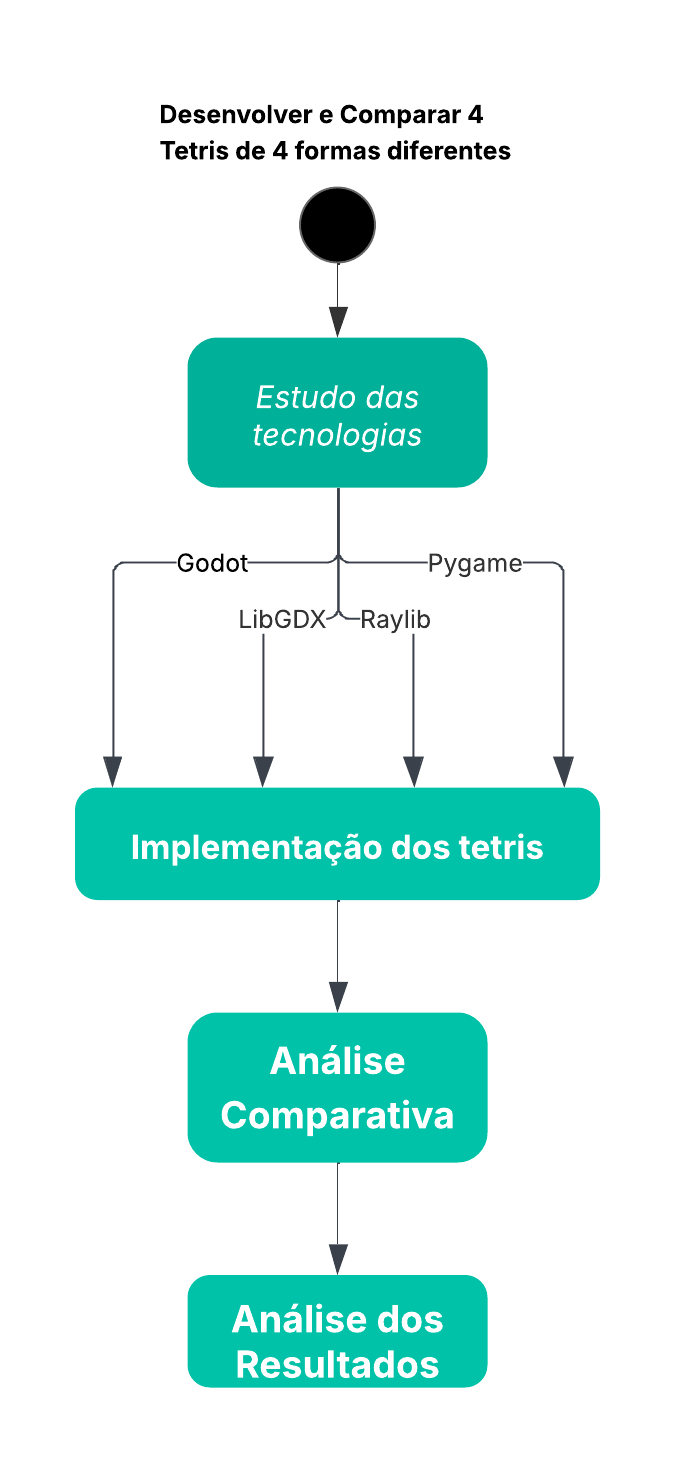
\includegraphics[scale=1.2]{imagens/DiagramaMetodologia.png}
	\\\textbf{Fonte:} Feito pelo autor
\end{figure}
\FloatBarrier

\begin{enumerate}
    \item \textbf{Estudos das tecnologias:} Para cada linguagem de programação e sua respectiva \textit{engine} e seus respectivos \textit{frameworks} 
    (\textit{Godot}, Pygame, Raylib, LibGDX)
    será feito um estudo inicial para aprender como funciona a estrutura de cada \textit{framework} e seus principais métodos, 
    o ciclo de vida de um jogo tanto da \textit{engine} como nos \textit{framework} é praticamente igual, com algumas diferenças entre si, o que
    tornará o processo de aprendizagem menos complexo. O estudo será feito de forma prática, consultando documentações oficiais e materias complementares conforme a necessidade do desenvolvimento, 
    a etapa do estudo das tecnologias e a implementação ocorrerá paralelamente.

    \item \textbf{Implementação dos \textit{Tetris}:} A escolha do jogo \textit{Tetris} para implementação e comparação foi por que é um jogo clássico de lógica simplificada,
    porém necessita recursos fundamentais que uma ferramenta de desenvolvimento de jogo oferece como por exemplo: renderização gráfica, detecção de colisão, manipulação de um array de duas
    dimensões,, controle do jogador, atualização de telas e outros.
    Será feita a implementação 
    
    \item \textbf{Análise comparativa:}
    \item \textbf{Resultado das análise:}
\end{enumerate}